%% file: template.tex = LaTeX template for article-like report 
%% init: sometime 1993
%% last: Feb  8 2015  Rob Rutten  Deil
%% site: http://www.staff.science.uu.nl/~rutte101/rrweb/rjr-edu/manuals/student-report/

%% First read ``latex-bibtex-simple-manual.txt'' at
%% http://www.staff.science.uu.nl/~rutte101/Report_recipe.html

%% Start your report production by copying this file into your XXXX.tex.
%% Small changes to the header part will make it an A&A or ApJ manuscript.

%%%%%%%%%%%%%%%%%%%%%%%%%%%%%%%%%%%%%%%%%%%%%%%%%%%%%%%%%%%%%%%%%%%%%%%%%%%%
\documentclass{aa}   %% Astronomy & Astrophysics style class

\usepackage{graphicx,natbib,url,twoopt}
\usepackage[varg]{txfonts}           %% A&A font choice
\usepackage{hyperref}                %% for pdflatex
%%\usepackage[breaklinks]{hyperref}  %% for latex+dvips
%%\usepackage{breakurl}              %% for latex+dvips
\usepackage{pdfcomment}              %% for popup acronym meanings
\usepackage{acronym}                 %% for popup acronym meanings

\hypersetup{
  colorlinks=true,   %% links colored instead of frames
  urlcolor=blue,     %% external hyperlinks
  linkcolor=red,     %% internal latex links (eg Fig)
}

\bibpunct{(}{)}{;}{a}{}{,}    %% natbib cite format used by A&A and ApJ

\pagestyle{plain}   %% undo the fancy A&A pagestyle 

%% Add commands to add a note or link to a reference
\makeatletter
\newcommand{\bibnote}[2]{\@namedef{#1note}{#2}}
\newcommand{\biblink}[2]{\@namedef{#1link}{#2}}
\makeatother

%% Commands to make citations ADS clickers and to add such also to refs
%% May 2014: they give error stops ("Illegal parameter number ..."}
%%   for plain latex with TeX Live 2013; the ad-hoc fixes added below let
%%   latex continue instead of stop within these commands.
%%   Please let me know if you know a better fix!
%%   No such problem when using pdflatex.
\makeatletter
 \newcommandtwoopt{\citeads}[3][][]{%
   \nonstopmode%              %% fix to not stop at error message in latex
   \href{http://adsabs.harvard.edu/abs/#3}%
        {\def\hyper@linkstart##1##2{}%
         \let\hyper@linkend\@empty\citealp[#1][#2]{#3}}%   %% Rutten, 2000
   \biblink{#3}{\href{http://adsabs.harvard.edu/abs/#3}{ADS}}%
   \errorstopmode}            %% fix to resume stopping at error messages 
 \newcommandtwoopt{\citepads}[3][][]{%
   \nonstopmode%              %% fix to not stop at error message in latex
   \href{http://adsabs.harvard.edu/abs/#3}%
        {\def\hyper@linkstart##1##2{}%
         \let\hyper@linkend\@empty\citep[#1][#2]{#3}}%     %% (Rutten 2000)
   \biblink{#3}{\href{http://adsabs.harvard.edu/abs/#3}{ADS}}%
   \errorstopmode}            %% fix to resume stopping at error messages
 \newcommandtwoopt{\citetads}[3][][]{%
   \nonstopmode%              %% fix to not stop at error message in latex
   \href{http://adsabs.harvard.edu/abs/#3}%
        {\def\hyper@linkstart##1##2{}%
         \let\hyper@linkend\@empty\citet[#1][#2]{#3}}%     %% Rutten (2000)
   \biblink{#3}{\href{http://adsabs.harvard.edu/abs/#3}{ADS}}%
   \errorstopmode}            %% fix to resume stopping at error messages 
 \newcommandtwoopt{\citeyearads}[3][][]{%
   \nonstopmode%              %% fix to not stop at error message in latex
   \href{http://adsabs.harvard.edu/abs/#3}%
        {\def\hyper@linkstart##1##2{}%
         \let\hyper@linkend\@empty\citeyear[#1][#2]{#3}}%  %% 2000
   \biblink{#3}{\href{http://adsabs.harvard.edu/abs/#3}{ADS}}%
   \errorstopmode}            %% fix to resume stopping at error messages 
\makeatother

%% Acronyms
\newacro{ADS}{Astrophysics Data System}
\newacro{NLTE}{non-local thermodynamic equilibrium}
\newacro{NASA}{National Aeronautics and Space Administration}

%% Add popups with meaning to acronyms 
%% NB: only show up in Adobe Reader and do not work with \input or \include
\gdef\acp#1{%
  \pdfmarkupcomment[markup=Underline,color={1 1 1},author={{#1}},opacity=0]%
  {{#1}}{{\acl{#1}}}}

%% Spectral species
\def\MgI{\ion{Mg}{I}}          %% A&A; for aastex use \def\MgI{\ion{Mg}{1}} 
\def\MgII{\ion{Mg}{II}}        %% A&A; for aastex use \def\MgII{\ion{Mg}{2}} 

%% Hyphenation
\hyphenation{Schrij-ver}       %% Dutch ij is a single character

%%%%%%%%%%%%%%%%%%%%%%%%%%%%%%%%%%%%%%%%%%%%%%%%%%%%%%%%%%%%%%%%%%%%%%%%%%%%
\begin{document}  

%% simple header.  Change into A&A or ApJ commands for those journals

\twocolumn[{%
\vspace*{4ex}
\begin{center}
  {\Large \bf N-body simulation of an open galactic cluster}\\[4ex]       
  {\large \bf Andreas Ellewsen(52), 
              Peder Forfang(55)}\\[4ex]
 \begin{minipage}[t]{15cm}
  {\bf Abstract.}  An open cluster is a typical phenomenon in our galaxies. It consists of a few thousand stars of roughly the same age. They are loosely bound by mutual gravitational attraction and can migrate, through internal close encounters, to the main body of the host galaxy. In this report we have created a simulation of an open cluster based on Newtonian gravity. We study how it evolves through time.

  \vspace*{2ex}
  \end{minipage}
\end{center}
}] 


%%%%%%%%%%%%%%%%%%%%%%%%%%%%%%%%%%%%%%%%%%%%%%%%%%%%%%%%%%%z%%%%%%%%%%%%%%%%%
\section{Introduction}     \label{sec:introduction}
%%%%%%%%%%%%%%%%%%%%%%%%%%%%%%%%%%%%%%%%%%%%%%%%%%%%%%%%%%%%%%%%%%%%%%%%%%%%
In this project we develop a code that performs simulations of an open cluster using Newtonian gravity. Since stars in these clusters are about the same age and material, many of the variable parameters are kept constant when compared to each other. Thus they make an interesting study of stellar evolution.
The programming languages used are C++ and Python. We use C++ for the calculations, and Python for generating plots and animations.
See section \ref{sec:codes} for a list of programs used.

First of we will consider the simple Newtonian two-body system. We would like to compare two different numerical approaches to this problem, namely the fourth order Runge Kutta method and the Velocity-Verlet method, to verify that our code works as intended, and to get an idea of which method we should  continue using in larger systems. We find that the Velocity-Verlet make a good candidate for larger simulations.

We continue to simulate an open cluster and extend our code to an arbitrary number of stars. We will consider a closed system, meaning it will not be affected by the environment outside of the cluster such as dust and other clouds. In such an over dense system it is natural to predict that it will eventually collapse, virialize and reach an equilibrium state. We will study the evolution of the cluster.
%%%%%%%%%%%%%%%%%%%%%%%%%%%%%%%%%%%%%%%%%%%%%%%%%%%%%%%%%%%%%%%%%%%%%%%%%%%%
\section{The two-body system}    \label{sec:twobody}
%%%%%%%%%%%%%%%%%%%%%%%%%%%%%%%%%%%%%%%%%%%%%%%%%%%%%%%%%%%%%%%%%%%%%%%%%%%%
The first step is to make a code that can simulate gravity between two bodies.
We choose to use the earth-sun system as a start since that gives a nice benchmark for our program.

The gravitational force on earth from the sun is 
\begin{equation}
 F_G = -G \frac{M_1 M_2}{R^2}
\end{equation}
which by using Newton's second law yields
\begin{equation}
 \overrightarrow{a_2} = -G \frac{M_1}{R^2}\frac{\overrightarrow{R_1}}{R}
\end{equation}
similarly the acceleration on the sun from earth is 
\begin{equation}
 \overrightarrow{a_1} = -G \frac{M_2}{R^2}\frac{\overrightarrow{R_2}}{R}
\end{equation}
where $\overrightarrow{R_1}$ is the vector pointing from the sun towards the earth, $\overrightarrow{R_2}$ is the other way, and $R = |R_1|=|R_2|$. 

Using both methods to calculate the velocity and position from this results in figures \ref{ES_1h_2y}-\ref{ES_1m_50y}. It is clear from the figures that Runge Kutta 4 is more stable than Velocity-Verlet for this system. While Velocity-Verlet starts to migrate outward with $\Delta t = 12$hours, Runge Kutta 4 stays in orbit with steps up to 2 weeks. Increasing the time step even further up to 1 month reveals that Runge Kutta stays in orbit (even if it is 12 sided polygon instead of an ellipse) for a very long time before it migrates inward, and gets thrown out when it gets so close that it gets an acceleration which it can not recover from in the next step.

%===========================================================================
\begin{figure}[hbtp]
 \centering
 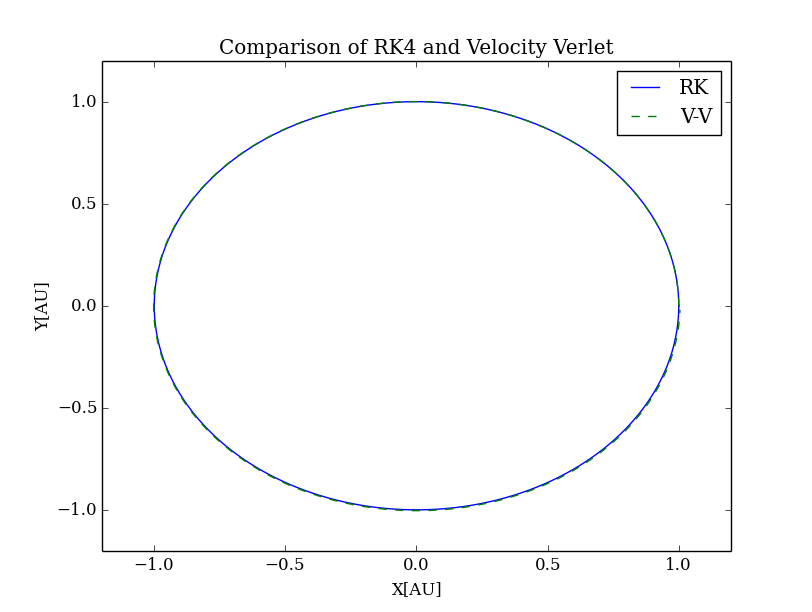
\includegraphics[width=80mm]{ES_1h_2y.png}
 \caption[]{\label{ES_1h_2y}
   Simulation of the earth-sun system for 2 years with a time step of 1 hour. 
 }
\end{figure}
\begin{figure}[hbtp]
 \centering
 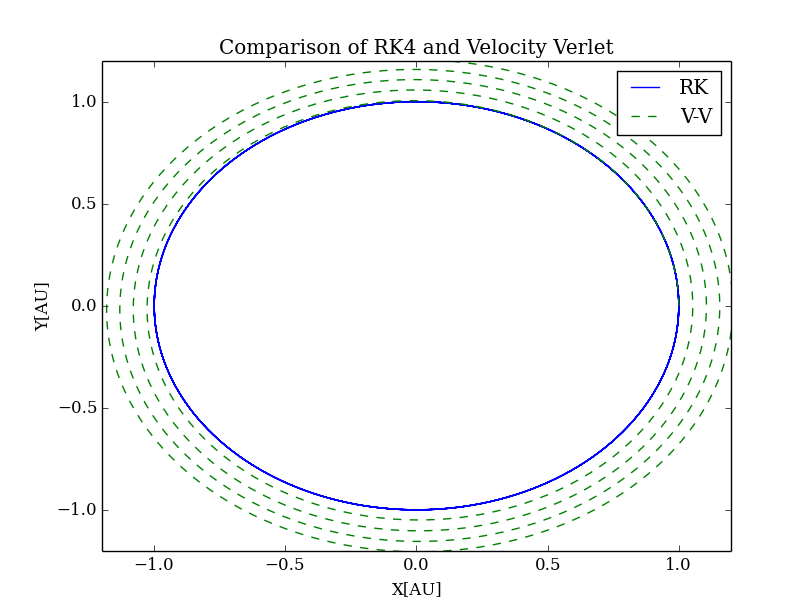
\includegraphics[width=80mm]{ES_0_5d_5y.png}
 \caption[]{\label{ES_0_5d_5y}
   Simulation of the earth-sun system for 5 years with a time step of 12 hours. 
 }
\end{figure}
\begin{figure}[hbtp]
 \centering
 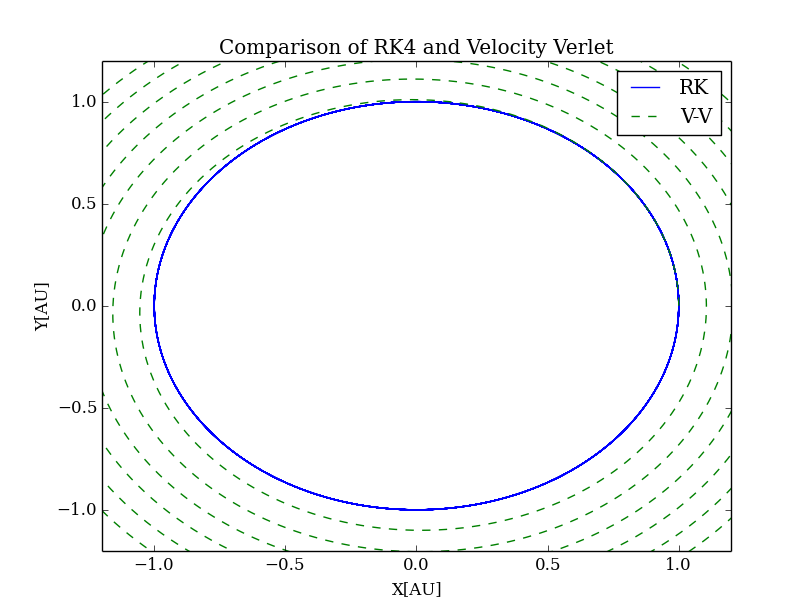
\includegraphics[width=80mm]{ES_1d_10y.png}
 \caption[]{\label{ES_1d_10y}
   Simulation of the earth-sun system for 10 years with a time step of 1 day. 
 }
\end{figure}
\begin{figure}[hbtp]
 \centering
 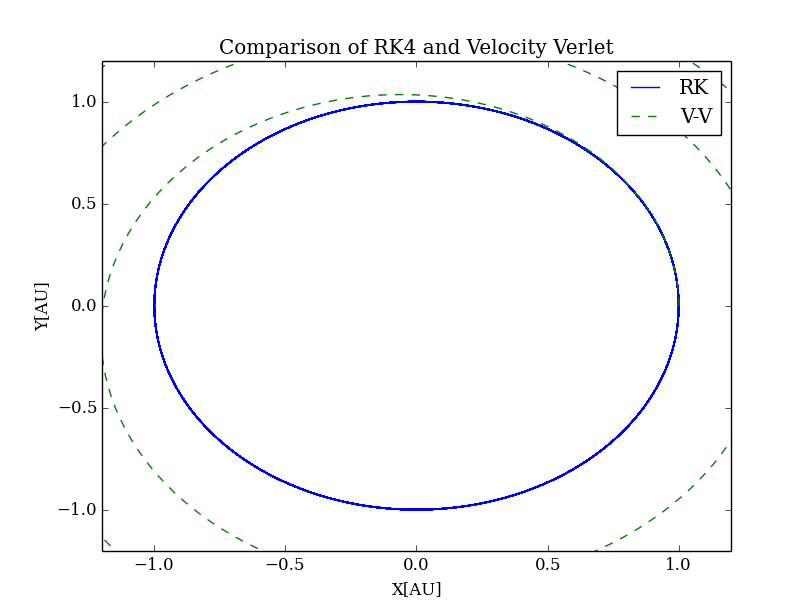
\includegraphics[width=80mm]{ES_3_5d_50y.png}
 \caption[]{\label{ES_3_5d_50y}
   Simulation of the earth-sun system for 50 years with a time step of 3.5 days. 
 }
\end{figure}
\begin{figure}[hbtp]
 \centering
 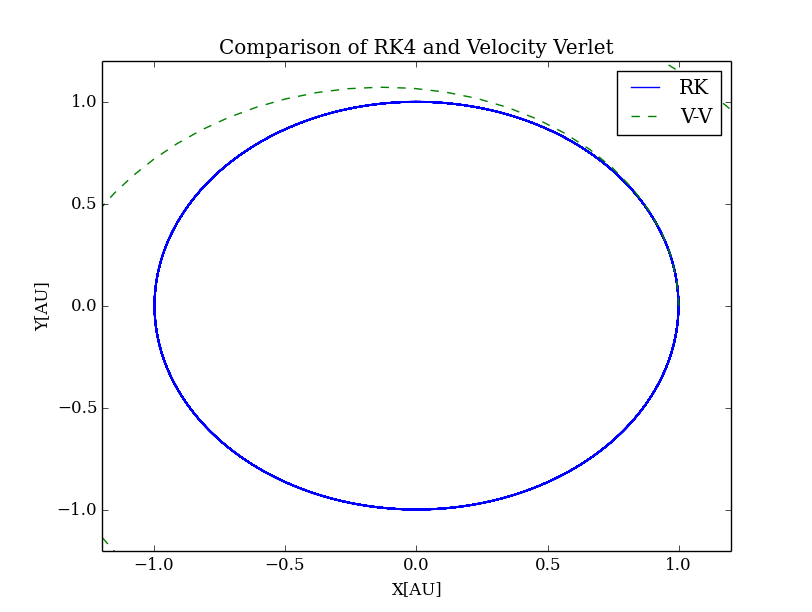
\includegraphics[width=80mm]{ES_7d_50y.png}
 \caption[]{\label{ES_7d_50y}
   Simulation of the earth-sun system for 50 years with a time step of 1 week. 
 }
\end{figure}
\begin{figure}[hbtp]
 \centering
 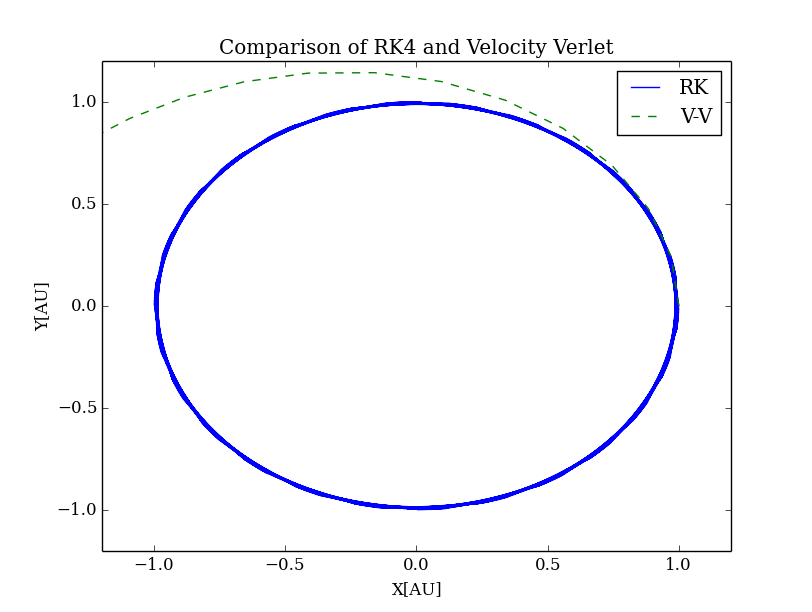
\includegraphics[width=80mm]{ES_14d_50y.png}
 \caption[]{\label{ES_14d_50y}
   Simulation of the earth-sun system for 50 years with a time step of 2 weeks.  
 }
\end{figure}
\begin{figure}[hbtp]
 \centering
 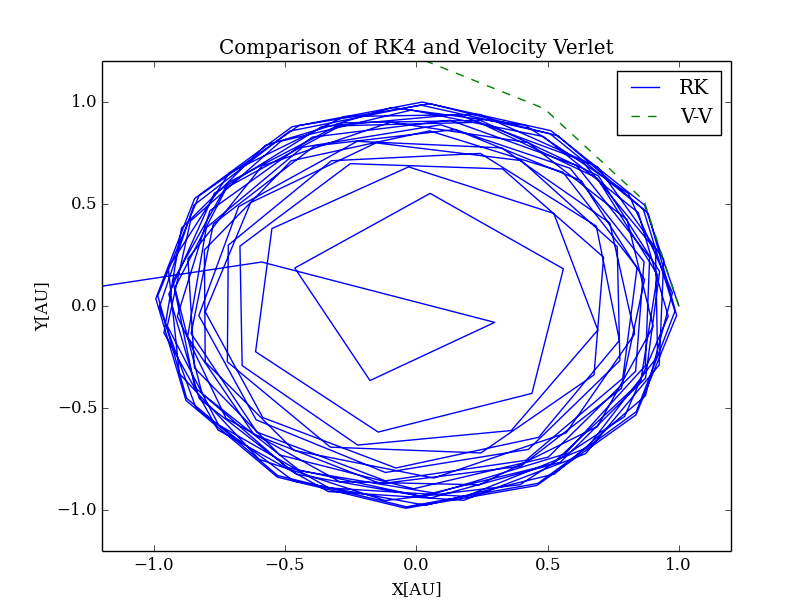
\includegraphics[width=80mm]{ES_1m_50y.png}
 \caption[]{\label{ES_1m_50y}
   Simulation of the earth-sun system for 50 years with a time step of 1 month.  
 }
\end{figure}

From this we can conclude that Runge Kutta 4 is more stable for large time steps than Velocity-Verlet. 
However, if Velocity-Verlet is much faster to calculate it may be better in the end for simulating many objects.

Setting the time step to be 1 day, and simulating for 20 years and measuring the average time one step takes shows that Runge Kutta 4 uses $0.0016$seconds per step, while Velocity-Verlet uses $0.0008$seconds per step. This indicates that Velocity-Verlet is twice as fast that compute. 
Doing the same with time step 2 days, and simulating for 20 years shows that Runge Kutta 4 uses $0.0009$ seconds, while Velocity-Verlet uses $0.00045$ seconds per step. This shows that Velocity-Verlet is still twice as fast as Runge Kutta 4.

However, it also shows that reducing the number of steps to half also reduces the time used for each step by approximately half as well. This indicates that there may be something slowing down the code in a part of the code not related to the methods. This is probably caused by the function that calculates the acceleration taking in the entire armadillo cube containing positions and velocities at all times. If this code is to be developed further after this project this is something that should be investigated to reduce computation times.

From this we can conclude that even though Velocity-Verlet is twice as fast, Runge Kutta 4 can use more than twice as large time steps, and thus simulate the same total time in less than half the time steps resulting in a faster total computation time. 

In this case one should use Runge Kutta 4. Note however that this does not say anything about conservation of energy in the system. If one wants to simulate the system for hundreds or thousands of years Velocity-Verlet is the way to go since that method is symplectic, which is not the case for Runge Kutta 4. 

The Verlet method is actually a second-order symplectic integrator, and there are higher order ones with better precision, but they need more computation time so we will stick with the Velocity-Verlet method.
%===========================================================================
%%%%%%%%%%%%%%%%%%%%%%%%%%%%%%%%%%%%%%%%%%%%%%%%%%%%%%%%%%%%%%%%%%%%%%%%%%%%
\section{N-body problem}    \label{sec:N-boy}
%%%%%%%%%%%%%%%%%%%%%%%%%%%%%%%%%%%%%%%%%%%%%%%%%%%%%%%%%%%%%%%%%%%%%%%%%%%%
Since we want to simulate an open cluster we need to extend our code to work on an arbitrary number of objects.
An open cluster is a group of up to a few thousand gravitationally bound stars created from the collapse of a molecular cloud.
To simulate this we should make our objects uniformly distributed inside a sphere of some radius $R_0$. Since the size of these clouds are on the light year scales we set $R_0 = 20$ ly. We choose to makes the masses of our objects follow a Gaussian distribution around 10 solar masses with a standard deviation of 1 solar mass. 

To make this dimensionless we need a time scale. A reasonable time scale to use would be the time it takes for a gravitationally bound structure of this size to collapse. The answer to this can be found in the Friedmann equations.
It turns out that the time it takes can be written
\begin{equation}
 \tau_{crunch} = \sqrt{\frac{3\pi}{32G\rho_0}}
\end{equation}
Note however that this assumes that our cluster is a continuous fluid, which would mean that $N \rightarrow \infty$.
If we actually calculate this time for 100 objects inside a sphere of radius $R_0$, with masses distributed around 10 solar masses we find that $\tau_{crunch} \approx 8$ million years.


Redefining our variables such that $\hat x = x/1ly$, $\hat r= r/1ly$, $\hat m = m/M_\odot$, and $\hat t = t/\tau_{crunch}$ means we can rewrite our equation for the acceleration on an object from another in the x dimension as 
\begin{equation}
\frac{d^2 \hat x}{d\hat t^2} = -\hat G \hat m \frac{\hat x}{\hat r^3}.
\end{equation}
The equations for the y and z direction look the same only changing $\hat x$ to $\hat y$ or $\hat z$.

Since we want to use $\tau_{crunch}$ as our time scale we set $\tau_{crunch} = 1$. This allows us to solve for $G$ resulting in 
$\hat G = \pi^2 R_0^3/8N\mu$, where $N$ is the number of objects, and $\mu$ the average mass of the objects. 

We simulate this system with both methods. See figures \ref{RK4N100dt0_001} and \ref{verletN100dt0_001}. These figures are quite crowded so it will probably be more interesting to watch the simulations of the system. See movies named 
$\mathrm{RK4N100dt0\_001.avi}$ and $\mathrm{verletN100dt0\_001.avi}$ in the project folder.
\begin{figure}[hbtp]
 \centering
 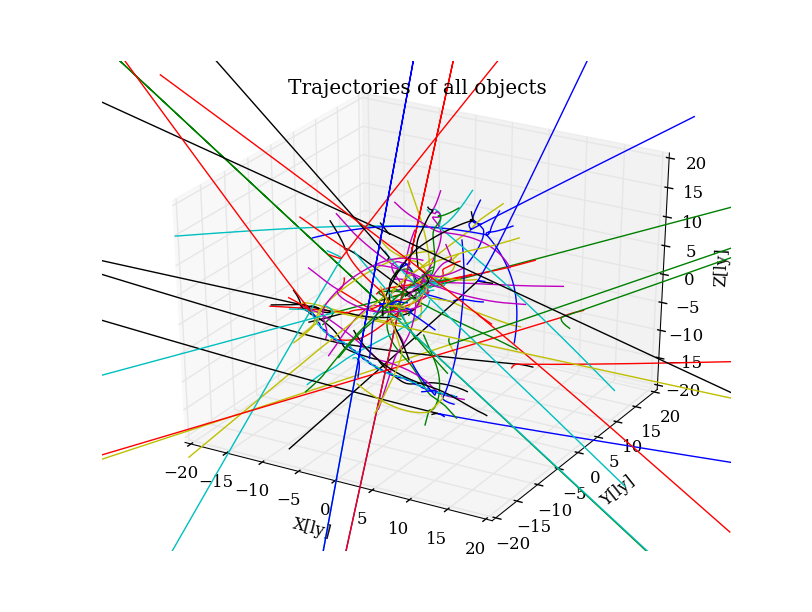
\includegraphics[width=80mm]{RK4N100dt0_001.png}
 \caption[]{\label{RK4N100dt0_001}
   Trajectories for 100 objects using time step 0.001$\tau_{crunch}$, simulating until $1.2\tau_{crunch}$. This simulation was done using Runge Kutta 4.
 }
\end{figure}
\begin{figure}[hbtp]
 \centering
 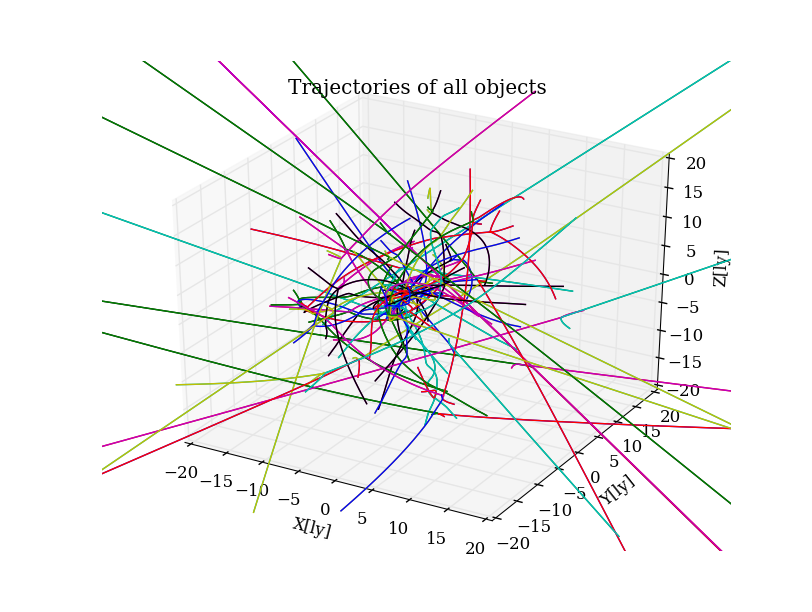
\includegraphics[width=80mm]{verletN100dt0_001.png}
 \caption[]{\label{verletN100dt0_001}
   Trajectories for 100 objects using time step 0.001$\tau_{crunch}$, simulating until $1.2\tau_{crunch}$. This simulation was done using Velocity-Verlet.
 }
\end{figure}

Now one may expect to see all the objects fall into a singularity at $t = \tau_{crunch}$. This does not happen, and it looks like they collapse later than that as well. Why is this the case? While using $\tau_{crunch}$ as a measure of the collapse time of the system works to a degree, our system does not have an infinite number of objects, and we don't have an infinite number of integration points in our simulation. Both of these facts contribute to us not observing a singularity in the model.

For this system watching the simulations or looking at the trajectories does not indicate that any of the methods is better than the other. 
Using Runge Kutta 4 we observe collapse around $t=1.2\tau_{crunch}$.
A lot of objects are ejected from the system. And it takes on average 0.009 seconds to advance one step.
Using Velocity-Verlet we observe the same.
There is however the point that it takes half the time to advance one step with Velocity-Verlet. 
We also know that Runge Kutta does not conserve energy while Velocity-Verlet does.

Since this will both save computation time and conserve the energy of the system we choose to continue with the Velocity-Verlet method.

It would be interesting to see if the system reaches an equilibrium after some time. To study this we run the simulation until $t=5\tau_{crunch}$. You can see the trajectories of the objects in figure \ref{verletN100dt0_001_Tcrunch5}. As expected this figure is quite crowded. It is easier to see what is happening by watching the video created from the simulation. This can be seen in the movie named $\mathrm{verletN100dt0\_001\_Tcrunch5.avi}$ in the project folder.

\begin{figure}[hbtp]
 \centering
 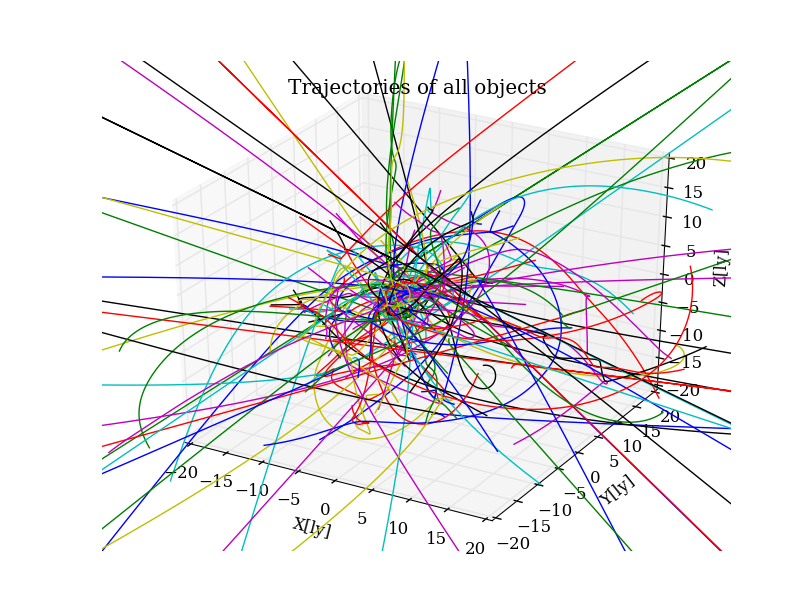
\includegraphics[width=80mm]{verletN100dt0_001_Tcrunch5.png}
 \caption[]{\label{verletN100dt0_001_Tcrunch5}
   Trajectories for 100 objects using time step 0.001$\tau_{crunch}$, simulating until $5\tau_{crunch}$. This simulation was done using Velocity-Verlet.
 }
\end{figure}

There is no clear equilibrium to be seen directly from the simulation. Since this is the case we choose to make a function that calculates the kinetic and potential energy of the system for each time step. Observing this through time should be a better indicator of whether the energy is conserved or not.

Calculating the kinetic, potential and total energy of the system for each time step returns figure \ref{energy1}. We see that the kinetic energy does some enormous jumps. This should coincide with the times objects get thrown out of the system in the simulation. Clearly the energy is not conserved because of these huge spikes in kinetic energy.
\begin{figure}[hbtp]
 \centering
 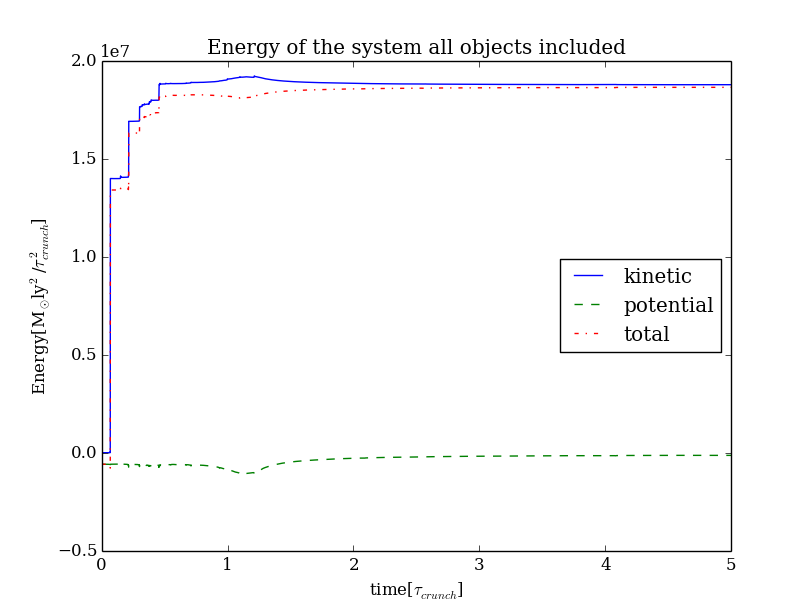
\includegraphics[width=80mm]{energy1.png}
 \caption[]{\label{energy1}
   The figure shows the energies of the system as a function of time. It is clear that energy is not conserved, and it is obvious that the objects that get thrown out of the system contribute very much to the kinetic energy. 
 }
\end{figure}
Since the kinetic energy of the objects that get thrown out distorts the energy of the system so much it would be interesting to see the behavior of the system if these were removed from the calculation. Figure \ref{energy2} shows exactly this. In this figure we have increased the simulation time again to see what happens for a few $\tau_{crunch}$. We see that if we exclude the objects which are eventually lost in the calculation of the energy, we get a peak in kinetic and potential energy around $1.1\tau_{crunch}$. This is a good sign that the energy function we have created functions properly. Note also that we do not end up with the same total energy at the end as we had at the beginning. This energy difference is caused by the objects that were thrown out of the system. These objects ``stole'' some of the energy from the bound objects before they left the system. For this simulation it amounts to approximately $E_{lost} = 2.16$ in units $10^5 M_\odot (ly)^2/\tau_{crunch}^2$. This amounts to approximately $70\%$ of the total energy.
Note also that the total energy stabilizes shortly after $\tau_{crunch}$. This is easily confirmed by looking at figure \ref{energy1} where we included all objects. This indicates that the systems stops throwing out objects after it reaches equilibrium.
\begin{figure}[hbtp]
 \centering
 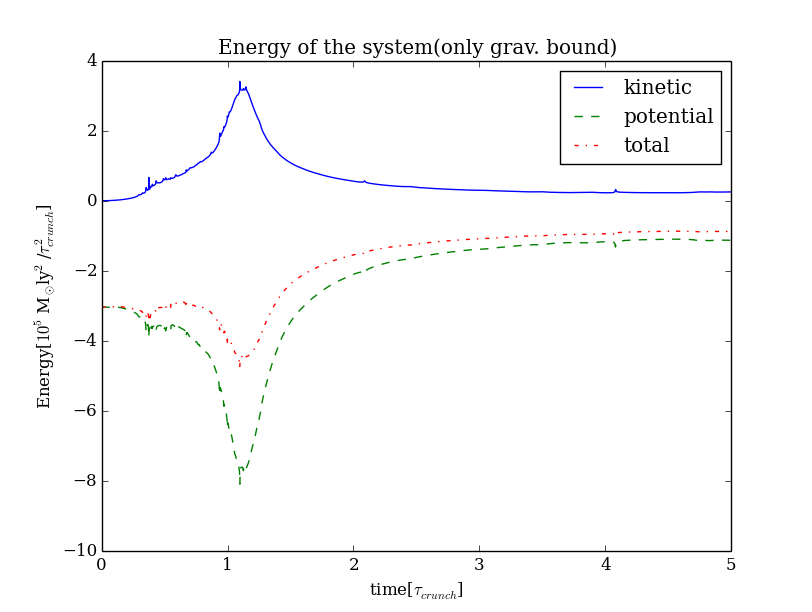
\includegraphics[width=80mm]{energy2.png}
 \caption[]{\label{energy2}
   The figure shows the energies for the system if one only includes the objects that were still gravitationally bound at the end of the simulation. We see a spike in the kinetic energy around $1.1\tau_{crunch}$. This is a bit lower than what we estimated by eye form the simulation. But this is of course more accurate.
 }
\end{figure}
Decreasing the number of objects to $N=50$ returns figures \ref{energy3} with all objects included, and figure \ref{energy4} where only the bound objects are included. For this simulation the energy lost is approximately $E_{lost} = 1.54$ in units $10^5 M_\odot (ly)^2/\tau_{crunch}^2$. This is an order of magnitude lower than for the system with $N=100$ but in contrast to the earlier system this amounts to about $85\%$ of the total energy the system started with.
\begin{figure}[hbtp]
 \centering
 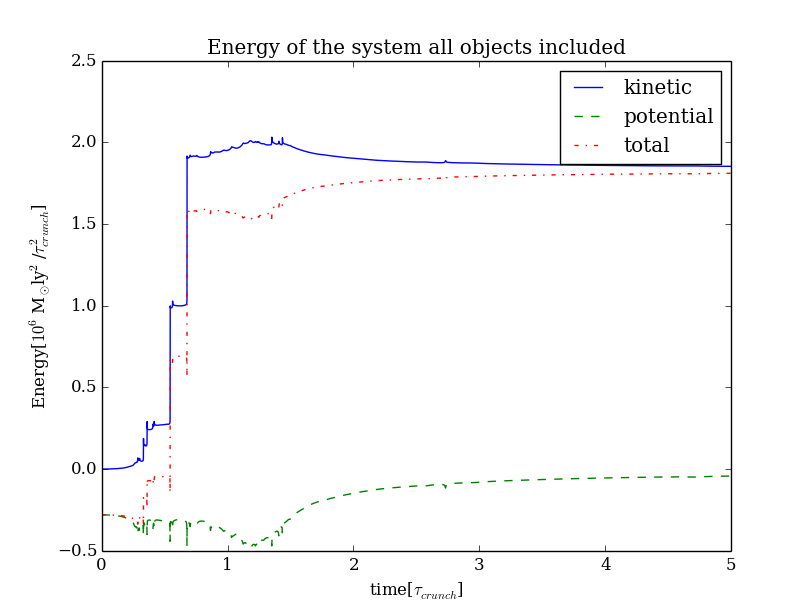
\includegraphics[width=80mm]{energy3.png}
 \caption[]{\label{energy3}
  In this figure we see the same behavior as we saw in the system with $N=100$. The kinetic energy of the ejected objects dominates. 
 }
\end{figure}
\begin{figure}[hbtp]
 \centering
 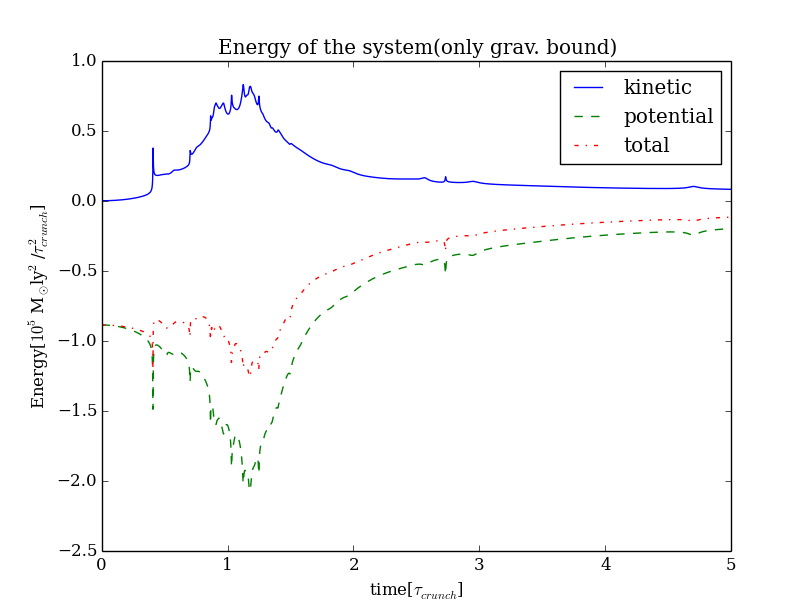
\includegraphics[width=80mm]{energy4.png}
 \caption[]{\label{energy4}
   The figure shows the energies for the system if one only includes the objects that were still gravitationally bound at the end of the simulation. We see a spike in the kinetic energy around $1.1\tau_{crunch}$. We see a slightly different form of the peak but it is still placed around the same time even if it is no. 
 }
\end{figure}
Doing the same experiment for a system with $N=200$ shows the same spike in kinetic energy early on, stabilizing at an equilibrium. See figure \ref{energy5}. The interesting thing here is as before the figure with only gravitationally bound objects counted. This is plotted in figure \ref{energy6}. We note that the curve is much smoother this time and we get a nice distinct peak at the same time as we have estimated earlier. There is still a substantial energy lost to the ejected objects. In this simulation the loss was $E_{lost} = 4.41$ in units $10^5 M_\odot (ly)^2/\tau_{crunch}^2$. This amounts to about $60\%$ of the total energy. 

\begin{figure}[hbtp]
 \centering
 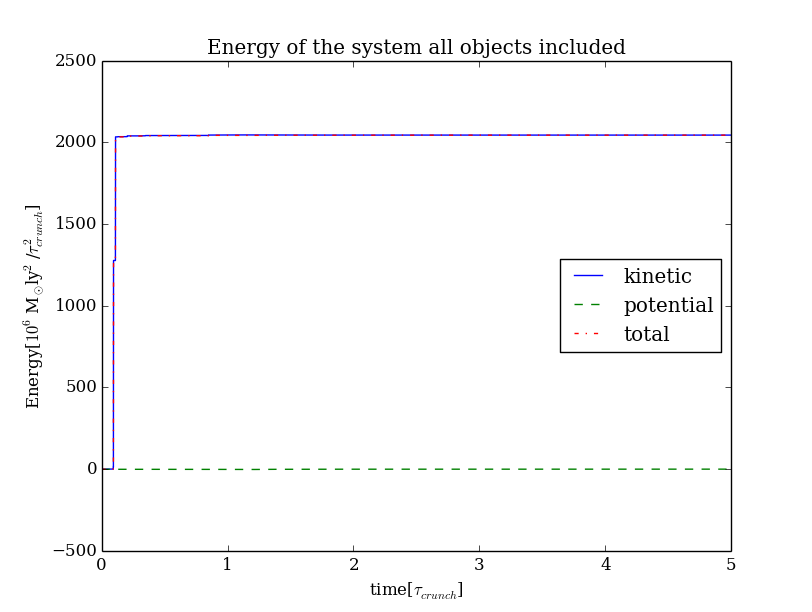
\includegraphics[width=80mm]{energy5.png}
 \caption[]{\label{energy5}
   In this figure we see the same behavior as we saw in the system with $N=50$ and $N=100$. The kinetic energy of the ejected objects dominates very early and because of this there is very little information to be extracted from the figure. 
 }
\end{figure}

\begin{figure}[hbtp]
 \centering
 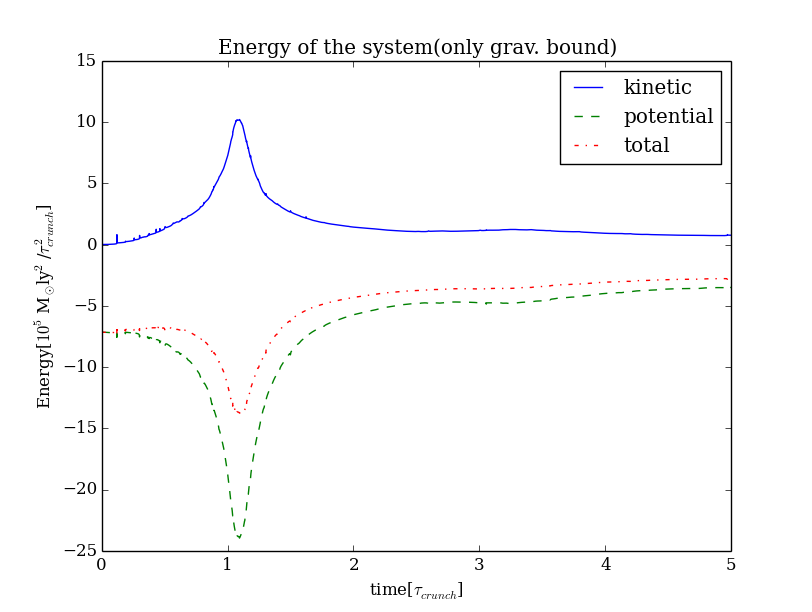
\includegraphics[width=80mm]{energy6.png}
 \caption[]{\label{energy6}
   The figure shows the energies for the system if one only includes the objects that were still gravitationally bound at the end of the simulation. We see a spike in the kinetic energy around $1.1\tau_{crunch}$. The peak in kinetic energy is still placed at the same place, but the graph as a whole is much smoother.
 }
\end{figure}
From this it would seem that increasing the number of objects decreases the fraction of energy lost to objects ejected from the system. However there is still an enormous loss of objects.

This loss of objects is caused by objects experiencing a large acceleration when they get too close to another object. Since we do not have infinitely small steps in time, this acceleration which should have lasted for a short time gets applied to the object for too long. To combat this numerical instability we introduce a smoothing function. There are many different methods  to introduce such a smoothing. In this project we choose to use a very simply one. Instead of using the regular Newtonian force law we will now use 
\begin{equation}
 F_{mod} = -G\frac{M_1 M_2}{r^2+\epsilon^2}.
\end{equation}
Where $\epsilon$ is a ``small'' constant.
The question now becomes, what $\epsilon$ value leads to the best energy conservation? And can we justify this value physically?

Trial and error leads us to conclude that we need $\epsilon \ge 0.01$ ly. This becomes clear by looking at the energy plots for the system when using different values. Figures \ref{Energy_N100_10Tcrunch_dt0_001_epsilon1}, \ref{Energy_N100_10Tcrunch_dt0_001_epsilon0_1}, and \ref{Energy_N100_10Tcrunch_dt0_001_epsilon0_01} show the energy for $\epsilon = 1, 0.1, 0.001$ respectively. 

\begin{figure}[hbtp]
 \centering
 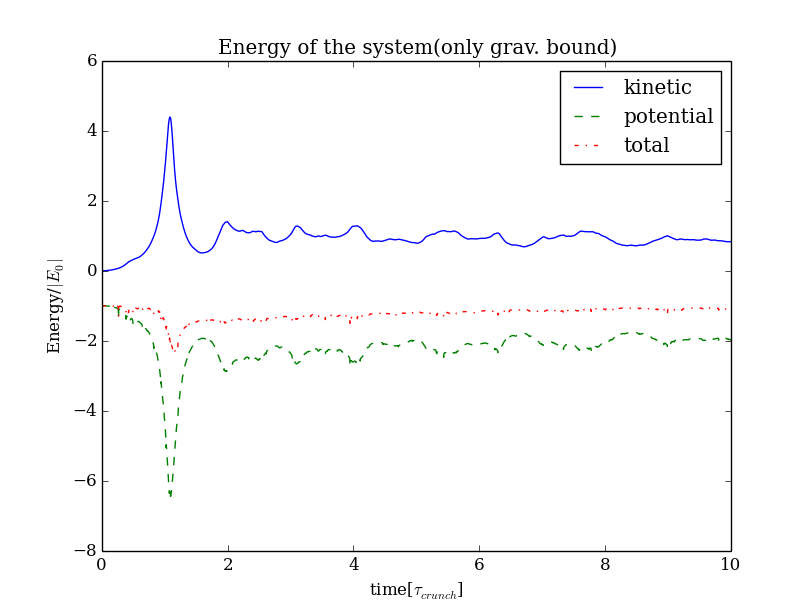
\includegraphics[width=80mm]{Energy_N100_10Tcrunch_dt0_001_epsilon1.png}
 \caption[]{\label{Energy_N100_10Tcrunch_dt0_001_epsilon1}
   The figure shows the energies for the system when we only include objects that were still bound at the end of the simulation. This is after we introduced the smoothing function. In this case we used $\epsilon = 1$. 
 }
\end{figure}

\begin{figure}[hbtp]
 \centering
 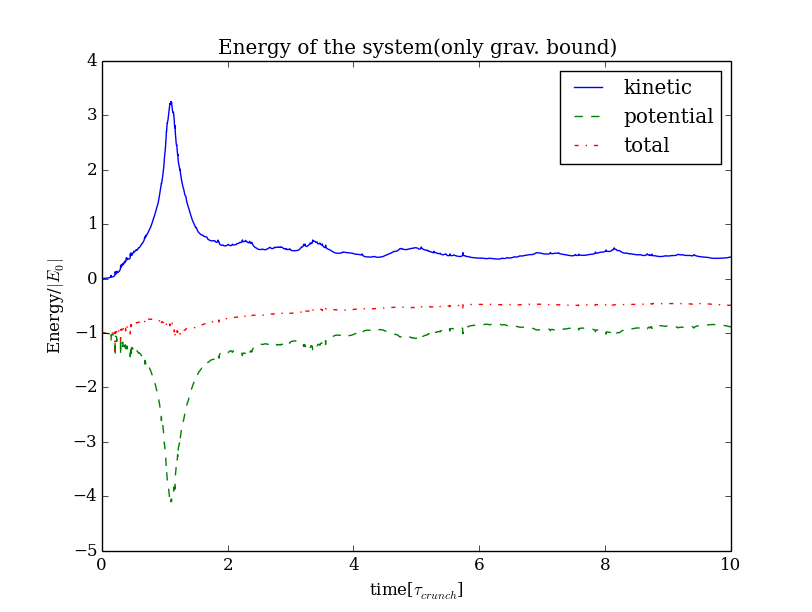
\includegraphics[width=80mm]{Energy_N100_10Tcrunch_dt0_001_epsilon0_1.png}
 \caption[]{\label{Energy_N100_10Tcrunch_dt0_001_epsilon0_1}
   The figures shows the same as the previous, but this is for $\epsilon = 0.1$.
 }
\end{figure}

\begin{figure}[hbtp]
 \centering
 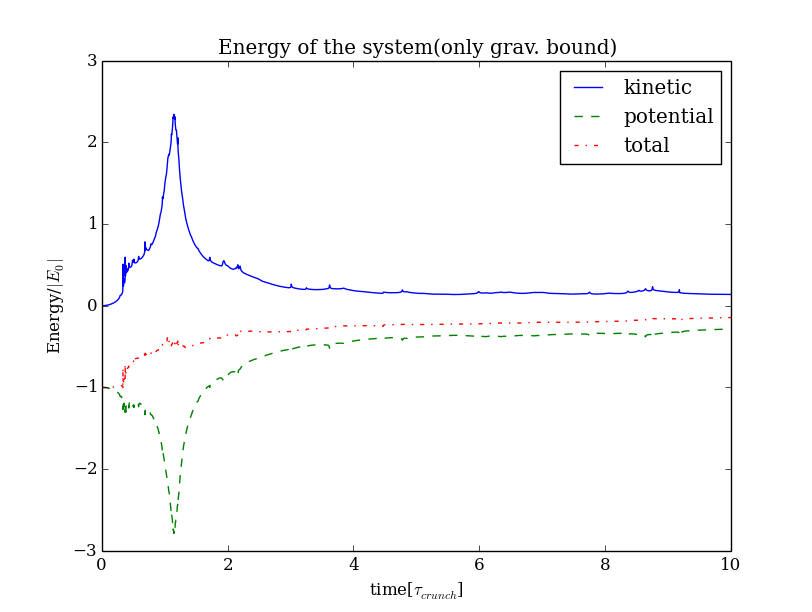
\includegraphics[width=80mm]{Energy_N100_10Tcrunch_dt0_001_epsilon0_01.png}
 \caption[]{\label{Energy_N100_10Tcrunch_dt0_001_epsilon0_01}
   The figures shows the same as the previous, but this is for $\epsilon = 0.01$.
 }
\end{figure}

By introducing the $\epsilon$ parameter we have made the system conserve energy better. Note however that the value we need is not easily justified physically. If one tries to argument that $\epsilon$ is a kind of minimum distance between the centers of two stars passing by each other, it breaks down since the distances we set it to are enormous. A quick calculation shows that $0.1 ly \approx 6300 AU$. If one looks at Betelgeuse, a red giant with a mass $M = 7.7-20 M_\odot$, it has a radius $R= 950-1200 R_\odot$. It is clear from this that the $\epsilon$ parameter can not be thought of as a kind of minimum distance between the objects. Instead we must conclude that it merely functions as an error correcting parameter to the error caused by finite time resolution. 

After our cluster has collapsed it will virialize around mass center.
The next step in this project is to look at the so called virial theorem.
The virial theorem simply states that for a bound gravitational system in equilibrium we have 
\begin{equation}
 2<K> = -<V>,
\end{equation}
where $<K>$ is the average (over time) kinetic energy of the system and $<V>$ is the average potential energy. We rearrange the equation to $2<K> + <V> = 0$ and divide by the initial total energy $E_0$. We expect this quantity to oscillate around 0 after the system virializes.
The smoothing parameter $\epsilon$ also affects whether the  theorem holds or not. We plot the virialization for the same $\epsilon$ values as we did previously. 

\begin{figure}[hbtp]
 \centering
 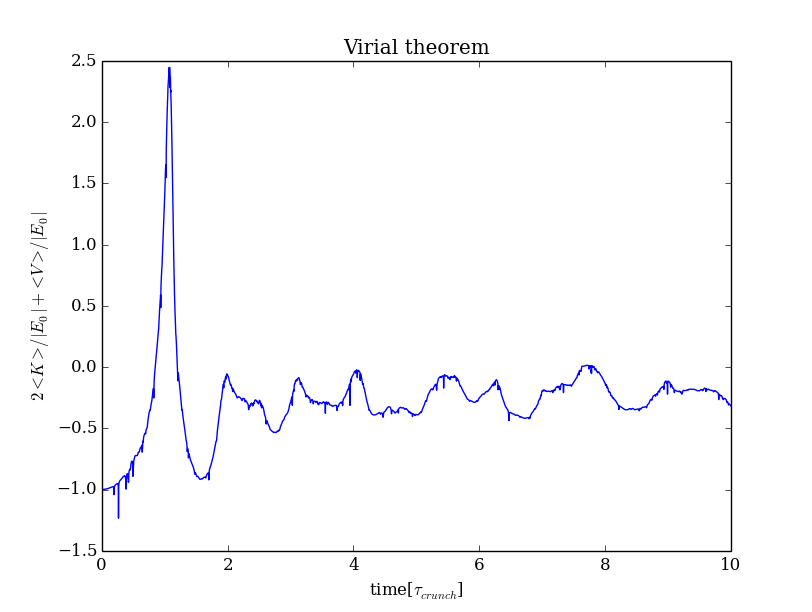
\includegraphics[width=80mm]{Virial_N100_10Tcrunch_dt0_001_epsilon1.png}
 \caption[]{\label{Virial_N100_10Tcrunch_dt0_001_epsilon1}
   This figure shows the quantity $2<K> + <V>$ for $\epsilon = 1$.
 }
\end{figure}


\begin{figure}[hbtp]
 \centering
 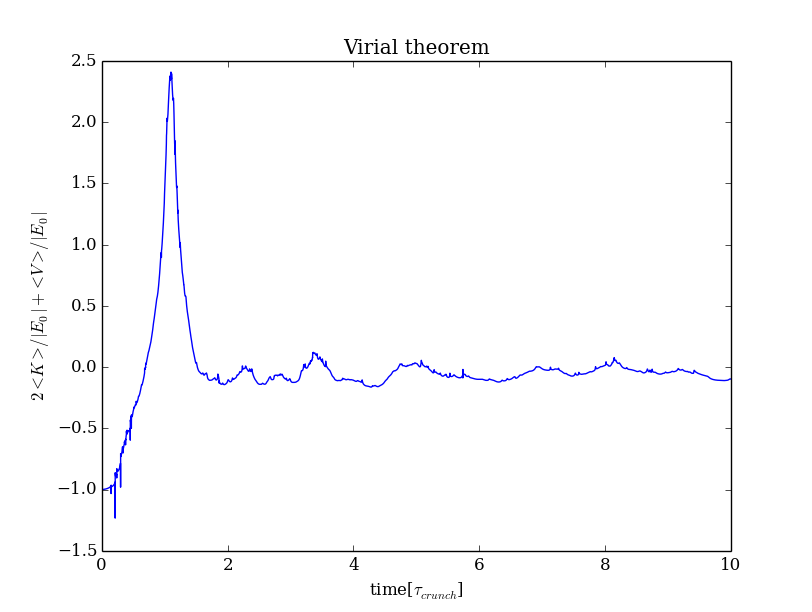
\includegraphics[width=80mm]{Virial_N100_10Tcrunch_dt0_001_epsilon0_1.png}
 \caption[]{\label{Virial_N100_10Tcrunch_dt0_001_epsilon0_1}
   This figure shows the quantity $2<K> + <V>$ for $\epsilon = 0.1$.
 }
\end{figure}

\begin{figure}[hbtp]
 \centering
 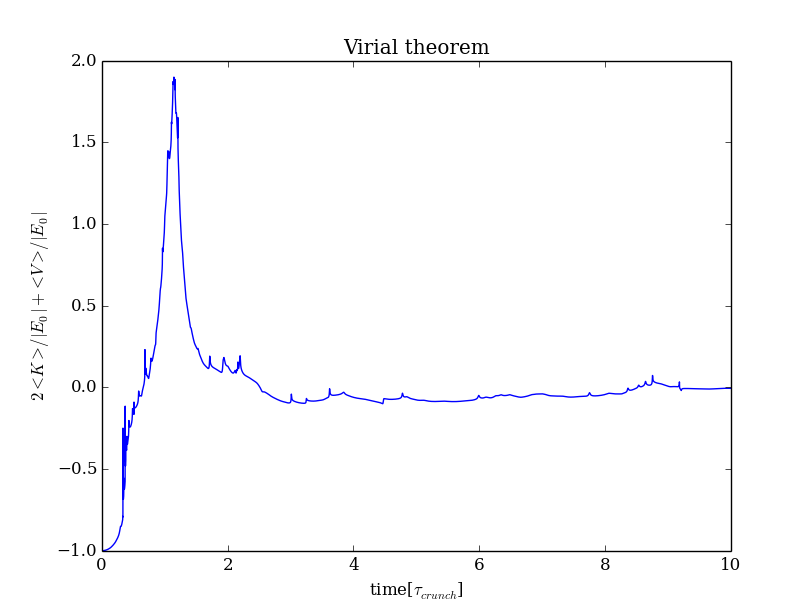
\includegraphics[width=80mm]{Virial_N100_10Tcrunch_dt0_001_epsilon0_01.png}
 \caption[]{\label{Virial_N100_10Tcrunch_dt0_001_epsilon0_01}
   This figure shows the quantity $2<K> + <V>$ for $\epsilon = 0.01$.
 }
\end{figure}



The effect of $\epsilon$ is shown in figures \ref{Virial_N100_10Tcrunch_dt0_001_epsilon1}, \ref{Virial_N100_10Tcrunch_dt0_001_epsilon0_1} and \ref{Virial_N100_10Tcrunch_dt0_001_epsilon0_01}. As we can see, it has the opposite effect on the virial theorem  than on energy conservation. For low $\epsilon$ the virialization is not affected, but as we increase the value to $\epsilon = 1$ we see that the graph starts oscillating around some other value than zero. This indicates that the virial theorem is no longer fulfilled.

The conclusion from this is that we get results that are both consistent with energy conservation and the virial theorem as long as we keep $\epsilon \approx 0.01$ ly. 

It would be interesting to study the number density of the objects in the halo.
To do this we calculate the mass center of the system and make a histogram of the number of objects within a radial distance in steps of 2 light years. The results is figure \ref{number_density_100}. However, this does not take into account that when increasing the distance form the center, each shell contains a larger volume than those closer to the center. When we take this into account we get figure \ref{number_density_100_scaled} where we have chosen to plot the number density for each distance range as a point half way between the distances. (The number density of objects between 0 and 2 light years is marked with a dot at 1 light years and so on). From this figure we see that we need a lot more objects to obtain any more information than that there seems to be a much larger number density close to the center of the system.
\begin{figure}[hbtp]
 \centering
 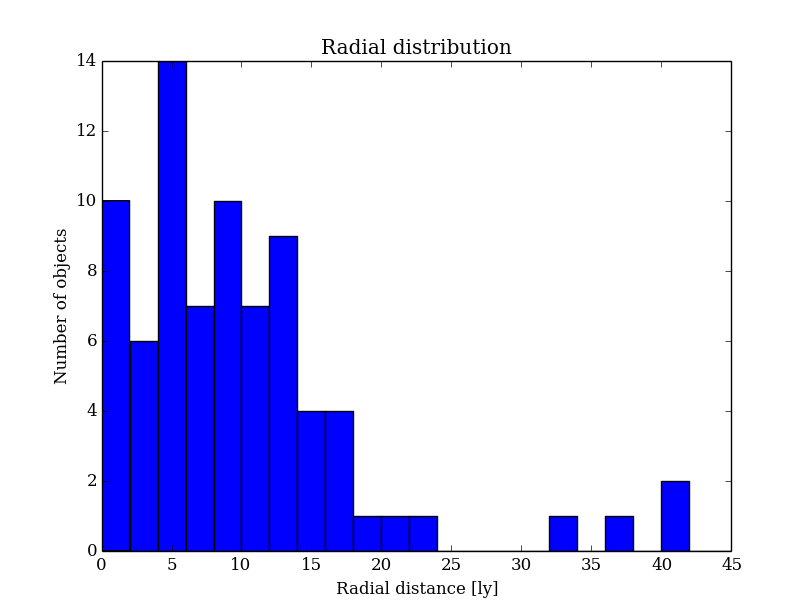
\includegraphics[width=80mm]{number_density_100.png}
 \caption[]{\label{number_density_100}
   Radial distribution of objects with $N=100$.
 }
\end{figure}

\begin{figure}[hbtp]
 \centering
 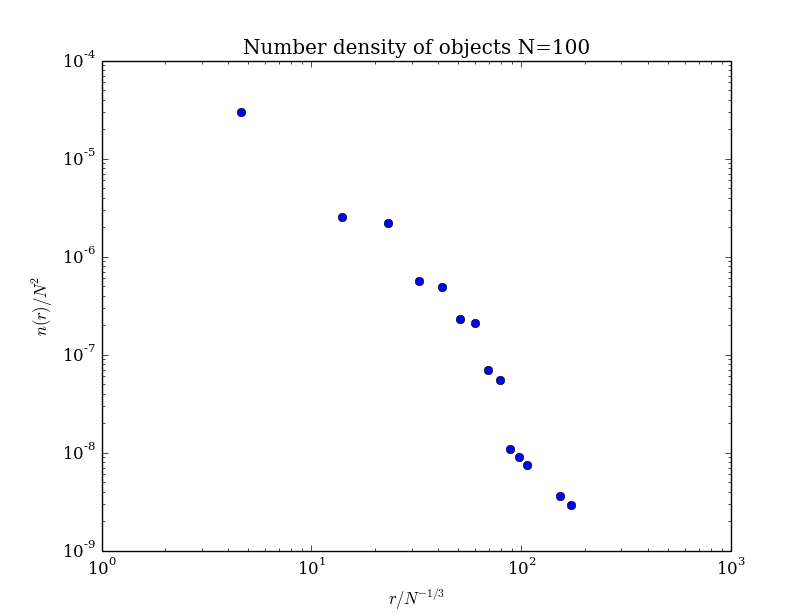
\includegraphics[width=80mm]{number_density_100_scaled.png}
 \caption[]{\label{number_density_100_scaled}
   Number of objects within given distances. It becomes clear than the number density is largest close to the mass center, and it diminishes quickly. 
 }
\end{figure}
The radial distribution of objects in this kind of cold collapse can often be fit very well with the simple expression
\begin{equation}
 n(r) = \frac{n_0}{1+ \big(\frac{r}{r_0}\big)^4}.
\end{equation}
Attempting to fit this to our curve reveals that setting $n_0 = 0.8$ and $r_0 = 1.5$ly works fairly well. The average distance from the mass center is $r_{avg} = 9.9$ly, with a standard deviation $\sigma = 8.5$.
See figure \ref{number_density_100_scaled_n}.
\begin{figure}[hbtp]
 \centering
 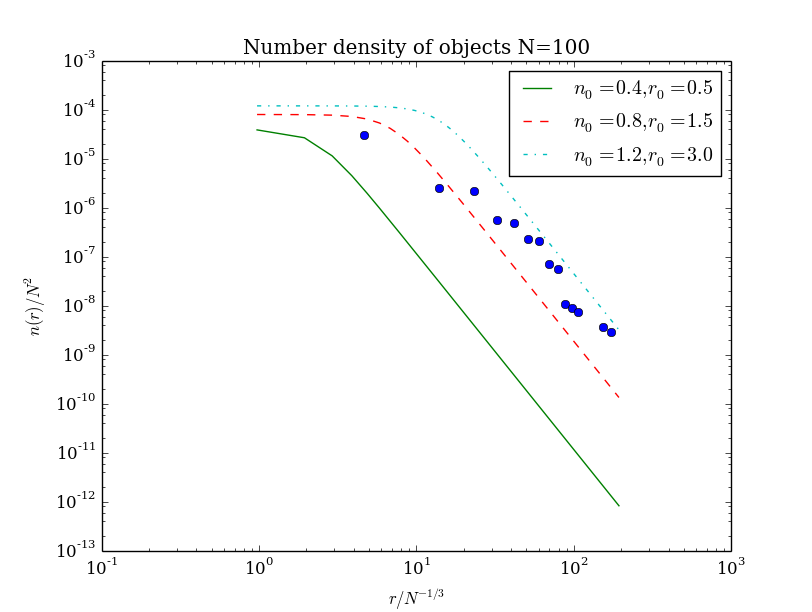
\includegraphics[width=80mm]{number_density_100_scaled_n.png}
 \caption[]{\label{number_density_100_scaled_n}
   Number density with a curve fit to the data. This is for $N=100$ objects.
 }
\end{figure}
It is still clear that we should increase the number of objects to get better data.
To save computation time we reduce the simulation time to $5\tau_{crunch}$. This is still well within the time frame after the system has virialized and reached equilibrium. With this setup we get an average distance $r_{avg} = 9.4$ly, and standard deviation $\sigma = 10.2$.
Figure \ref{number_density_500_scaled_n} shows the number density scaled with $N^2$ as a function distance scaled by $N^{-1/3}$. From the figure we see that the curve with $n_0 = 0.9$ and $r_0 = 3$ is the best fit.
\begin{figure}[hbtp]
 \centering
 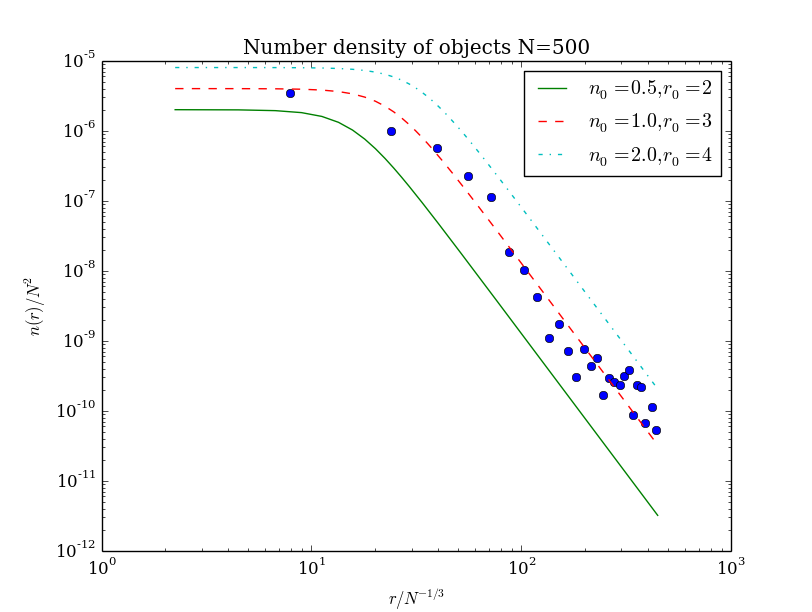
\includegraphics[width=80mm]{number_density_500_scaled_n.png}
 \caption[]{\label{number_density_500_scaled_n}
   Number density with curves to fit the data. This is for $N=500$ objects.
 }
\end{figure}
\begin{figure}[hbtp]
 \centering
 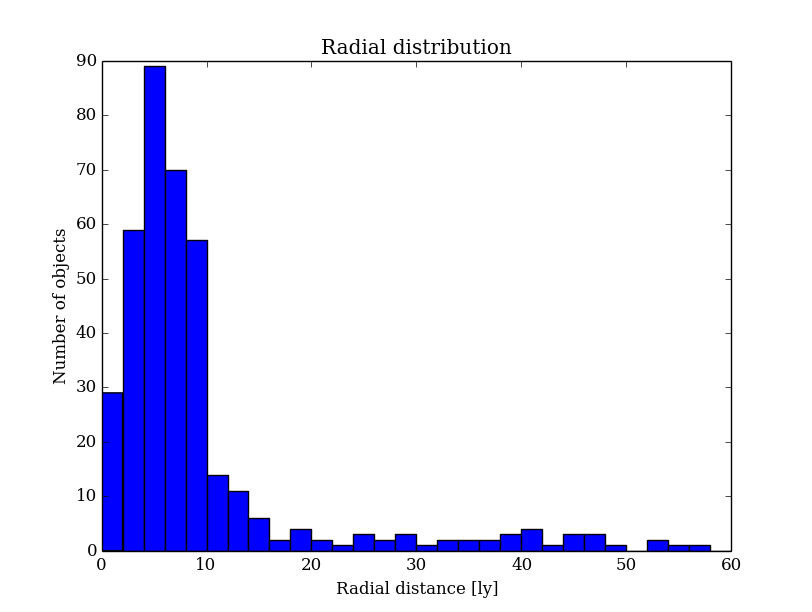
\includegraphics[width=80mm]{number_density_500.png}
 \caption[]{\label{number_density_500}
   Radial distribution of objects with $N=500$.
 }
\end{figure}

Unfortunately the computer we are using can not handle any more objects than this. Not only does the computation time increase too much. There is not enough memory to read the data files using python.
Because of this we are unable to find many $n_0$ and $r_0$ values for different numbers of objects $N$.

%%%%%%%%%%%%%%%%%%%%%%%%%%%%%%%%%%%%%%%%%%%%%%%%%%%%%%%%%%%%%%%%%%%%%%%%%%%%
\section{Methods}    \label{sec:methods}
%%%%%%%%%%%%%%%%%%%%%%%%%%%%%%%%%%%%%%%%%%%%%%%%%%%%%%%%%%%%%%%%%%%%%%%%%%%%
\subsection{Runge Kutta 4th order}
The Runge-Kutta of 4th order is a method of numerically integrating ordinary differential equations. A collaboration between calculations in intermediate steps of an interval cancel out the lower order error terms. The final step is obtained by using Simpson's rule, integrating at $t+\Delta t/2$. It can be approximated by
\begin{equation}
\int_t^{t+\Delta t} f(t,x) dt \approx \frac{1}{6}h(f(t,x) + 4f(t+ \frac{1}{2}h, x+ \frac{1}{2}h) + f(t + h, x + h)
\end{equation}
where h is the step length. 

Numerically, the RK4 can be implemented by four steps, each step slightly improves the accuracy by using the result from previous steps.

First, we use Euler's method to compute step $f(t,x)$ 
\begin{equation}
k1 = hf(t, x)
\end{equation}

Second, similar to the first step, only this time we compute the slope at the midpoint.

\begin{equation}
k2 = hf(t + \frac{1}{2}h, x + \frac{1}{2} k1)
\end{equation}

Again we compute the midpoint slope, but improve it by using our previous result k2.

\begin{equation}
k3 = hf(t + \frac{1}{2} h, x + \frac{1}{2} k2)
\end{equation}

The fourth step then calculates the step $x(t+\Delta t)$ by

\begin{equation}
k4 = hf(t + h, x +k3)
\end{equation}

The final step can then be computed:

\begin{equation}
x(t + h) = x(t) + \frac{1}{6}(k1 + 2k2 + 2k3 + k4)
\end{equation}

\subsection{Velocity-Verlet}
Another approach to integrate Newtons equation of motion is by the method Velocity-Verlet. This algorithm is very similar to the Euler method. The only difference is that the Velocity Verlet calculates an intermediate midpoint velocity step. 

\begin{equation}
v(t+\frac{1}{2}\Delta t) = v(t) + \frac{1}{2}a(t)\Delta t
\end{equation}

This midpoint velocity step is calculated using the acceleration derived from the interacting potential at the present position. With this velocity the next position is calculated.

\begin{equation}
x(t+\Delta t) = x(t) + v(t+\frac{1}{2}\Delta t)\Delta t
\end{equation}

The methods are similar up to this point. From here we derive a new acceleration $a(t+\Delta t)$ with the new position, and finally the next step velocity.

\begin{equation}
v(t+\Delta t) = v(t+\frac{1}{2}\Delta t) + \frac{1}{2}a(t+\Delta t)
\end{equation}

In the long term, this extra step improves the result. The Velocity Verlet also has an advantage over RK4. It calculates half the amount of steps as RK4 and thus takes half the time to finish. 
%%%%%%%%%%%%%%%%%%%%%%%%%%%%%%%%%%%%%%%%%%%%%%%%%%%%%%%%%%%%%%%%%%%%%%%%%%%%
\section{Conclusions} \label{sec:conclusions}
%%%%%%%%%%%%%%%%%%%%%%%%%%%%%%%%%%%%%%%%%%%%%%%%%%%%%%%%%%%%%%%%%%%%%%%%%%%%
We decided that the best numerical approach for our case was by using the Velocity-Verlet method. The reason for this was that the fourth order Runge Kutta, although close to perfect at small time steps, turned out to lose energy as we used appropriate time steps for our large scale system. Quite opposite, the Velocity-Verlet is not as accurate in computing the various trajectories, but the method is symplectic and thus conserves energy. 

Open clusters are key to understanding stellar evolution. Through internal close encounters stars gain momentum and are ejected out of the cluster. Our simulation lasts over large time scales. To complete the computations in reasonable time the time steps cannot be too small. As a consequence, a numerical instability arise. At close interactions stars gain massive acceleration which last for too long. The result was that they got ejected out of the cluster. We introduced a smoothing function as a simple numerical trick to fix this problem. This trick involved modifying the gravitational force with a constant $\epsilon$. We found that to minimize the disruption of other parameters the best value was $\epsilon = 0.1$. 

In our study we have found that the ejected mass and energy loss decreases as we apply more objects to our system. The remaining cluster collapses and starts to virialize. At this point it has reach an equilibrium and is stable against further loss. In reality most clusters are located in the galactic plane and will be exposed to radiation pressure, dust and other environmental forces. These external disruptions can cause instability in the cluster and may catalyze further ejections. 

We obtained our best resolution when we randomly distributed 500 objects inside a sphere of radius 20 light years. It takes about 8 million years to collapse. After virialization, most of the remaining objects is located inside a radius of 10 light years. The object farthest away is at 58 light years. In comparison, observed open clusters have a radius up to 180 light years. However, apart from environmental forces, these clusters have up to a few thousand stars. 

%%%%%%%%%%%%%%%%%%%%%%%%%%%%%%%%%%%%%%%%%%%%%%%%%%%%%%%%%%%%%%%%%%%%%%%%%%%%
\section{Codes} \label{sec:codes}
%%%%%%%%%%%%%%%%%%%%%%%%%%%%%%%%%%%%%%%%%%%%%%%%%%%%%%%%%%%%%%%%%%%%%%%%%%%%
Here follows a list of programs used to generate our results.
The main program that runs functions found in main.cpp and p5funcs.cpp
\begin{itemize}
\item main.cpp - main program
\item p5funcs.cpp - functions to solve problem
\item lib.cpp - library file
\item $\mathrm{earthsun\_plot.py}$ - plots earth-sun system (method 0)
\item energyplot.py - plots energy of system
\item $\mathrm{mass\_plot.py}$ - plots mass distribution
\item $\mathrm{position\_plot.py}$ - plots position and saves image files to folder
\item moviecreator.py - creates movie from image files in same folder
\item $\mathrm{radial\_density.py}$ - plots radial density
\end{itemize}
Video files: 
\begin{itemize}
\item $\mathrm{RK4N100dt0\_001.avi}$
\item $\mathrm{verletN100dt0\_001.avi}$
\item $\mathrm{verletN100dt0\_001\_5Tcrunch.avi}$
\end{itemize}

%%%%%%%%%%%%%%%%%%%%%%%%%%%%%%%%%%%%%%%%%%%%%%%%%%%%%%%%%%%%%%%%%%%%%%%%%%%%
\section{References} \label{sec:ref}
%%%%%%%%%%%%%%%%%%%%%%%%%%%%%%%%%%%%%%%%%%%%%%%%%%%%%%%%%%%%%%%%%%%%%%%%%%%%
\begin{itemize}
\item Morten Hjorth-Jensen, Computational Physics, Lecture notes Fall 2015 (2015)
\item Øystein Elgarøy, AST4220: Cosmology I (2009)
\item M. Joyce, B. Marcos, and F. Sylos Labini, Cold uniform spherical collapse revisited, AIP Conf. Proc. 1241, 955 (2010),[http://arxiv.org/abs/1011.0614].
\item http://www.fisica.uniud.it/~ercolessi/md/md/node21.html
\end{itemize}
%% references
%\bibliographystyle{aa-note} %% aa.bst but adding links and notes to references
%%\raggedright              %% only for adsaa with dvips, not for pdflatex
%\bibliography{XXX}          %% XXX.bib = your Bibtex entries copied from ADS

\end{document}

